\label{sec:examples_figures}
Figures should automatically be adjusted by the template. Table~\ref{table:figure_format} shows the important rules and Fig.~\ref{fig:example_figure} provides an example.

%Table: Figure format
\begin{table}[H]
    \centering
\begin{threeparttable}[H]
    \renewcommand{\arraystretch}{1.3}
    \caption{Figure format}
    \label{table:figure_format}
    \setlength\tabcolsep{5pt}
    \begin{tabular}{|l|l|l|}\hline
        \tableheader Item &\tableheader LUH &\tableheader SPbPU \\\hline

        Title Font        &Normal      &Italic\\\hline
        Title Location    &Below       &Below\\\hline
        Title Alignment   &Centered    &Centered\\\hline
        Number            &7.3         &7.3\\\hline
        Seperator         &:           &-\\\hline

    \end{tabular}
\end{threeparttable}
\end{table}

%Figure: Black Box Model
\begin{figure}[H]
    \centering
    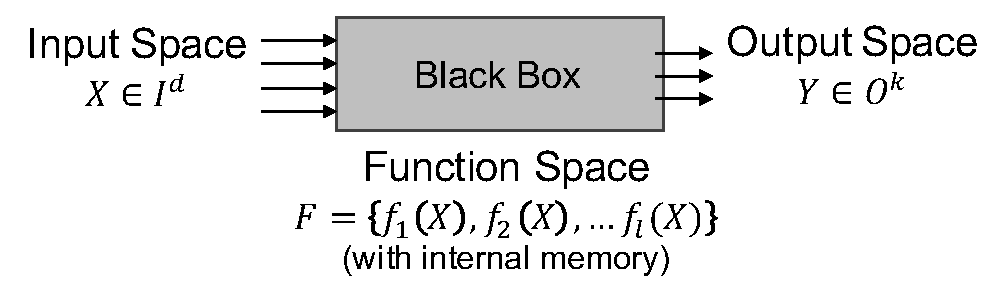
\includegraphics[width=0.9\columnwidth]{figures/blackbox_model.pdf}
    \vspace*{-4mm}
    \caption{Example figure}
    \label{fig:example_figure}
\end{figure}